\documentclass{beamer}
\usepackage[utf8]{inputenc}
\usepackage{pgf,tikz}
\usetikzlibrary{arrows}
\usetikzlibrary{matrix,chains,positioning,decorations.pathreplacing,arrows}
\usepackage{xcolor}
\usepackage{times}
\usepackage{amsmath}
\usepackage{verbatim}
\usepackage{hyperref}
%\usepackage[colorlinks=true,urlcolor=blue]{hyperref}
\usepackage{pdfpages}
\usepackage{hyperref}
\usepackage{graphicx,grffile}
\usepackage{verbatimbox}
% \usepackage{float}
% \usepackage{caption}
% \usepackage{subcaption}

%\usetheme{CambridgeUS} %Good
\setbeamertemplate{itemize item}[ball]
\setbeamertemplate{itemize subitem}[ball]

%\usepackage{enumerate}
%\numberwithin{equation}{section}


\title{Multiple-response models for multivariate binary response}
\author{Steve Cygu \& Prof. Jonathan Dushoff\\ \vspace{1cm} McMaster University, Canada.}
\date{April 09, 2019}

\begin{document}
\frame{\titlepage}

\frame{\small{\frametitle{OUTLINE}\tableofcontents}} 


\section{Background}

\begin{frame}{Background}
\begin{itemize}[<+->]
\item Longitudinal (2003 - 2015) NUHDSS covering Korogocho and Viwandani
\item Predictors
\begin{itemize}[<+->]
\item Slum area
\item Interview year
\item Age
\item Gender
\item Ethnicity
\item Household size
\item Wealth index
\item Household expenditure
\end{itemize}
\item Response(s): Three WASH variables were created as per WHO definition

\begin{itemize}[<+->]
\item Drinking water source
\item Toilet facility type
\item Garbage disposal method
\end{itemize}
\end{itemize}

\end{frame}


\section{Objective}

\begin{frame}{Objective}
The aim is to investigate the contribution of demographic, socialland economic factors to improved waster, sanitation and hygien (WASH) among the urban poor.
\end{frame}

\begin{frame}{Problems}
How do we account for the repeated measurements within the households across the years?
\begin{itemize}[<+->]
\item Model the wash variables separately (Manuscript already submitted?)
\item Pick one of the WASH indicator and treat the remaining two as fixed covariates
\end{itemize}
\pause
\textcolor{red}{The two approaches are not accounting for the unmeasured variations and correlation among the WASH variables} 
\end{frame}

\begin{frame}{Problems}
Does this matter?

\begin{itemize}[<+->]
\item Access to any of the WASH indicators (variables) vary within the households and also across the years.
\end{itemize}
\pause
\begin{columns}[t]
\column{.35\textwidth}
\includegraphics[width=\textwidth]{water_plot.pdf}
\pause
\column{.35\textwidth}
\includegraphics[width=\textwidth]{toilet_plot.pdf}
\pause
\column{.35\textwidth}
\includegraphics[width=\textwidth]{garbage_plot.pdf}
\end{columns}
\end{frame}

\begin{frame}{Problems}

There are several questions we can ask:
\begin{itemize}[<+->]
\item[1.] How do we pull information from (across) the three levels (WASH)?
\begin{itemize}[<+->]
\item Can we account for household level variations?
\end{itemize}
\item[2.] Can we estimate the correlation between the WASH variables while controlling for the other covariates?
\item[3.] Can we control for the variation and still get a reliable estimate of the covariance?
\end{itemize}

\pause
What we may know?
\begin{itemize}[<+->]
\item \textcolor{red}{This is a difficult problem}!!!
\item \textcolor{gray}{Generalised linear mixed effects models may be a good starting point}
\item But we need some understanding of data generation process
\begin{itemize}[<+->]
\item \textcolor{blue}{Some simulations}
\end{itemize}
\end{itemize}

\end{frame}

\section{Methods}
\begin{frame}{Methods}
Assume that we only observed the predictors and simulate response
\begin{itemize}[<+->]
\item Pick one of the predictors - \textcolor{blue}{wealth index}, $x$
\item There are some unobserved confounders, $U$, effect
\item Assume we know the effect sizes, $\beta$s
\pause
\[
\hat{y}_i = U_i + \beta_{0i} + \beta_{1i}x
\]
Where $i\in\{\text{WASH}\}$
\item Let $P$ be the probability that HH has access to $i\in\{\text{WASH}\}$
\[
P = \frac{1}{1 + \exp{(-\hat{y_i})}}
\]
\item Simulate response, $y_i$ from a binomial distribution with probability of observing WASH $P$
\end{itemize}
\pause
\textcolor{blue}{Now that we know the observed $\beta$s, can we find a model which gives us back the $\beta$s having answered the 3 question above?}
\end{frame}

\subsection{Simulations}
\begin{frame}{Simulation results}
\centering
\includegraphics[scale=0.4]{git_push/prop_plot.pdf}
\end{frame}

\subsection{Model fitting}

\begin{frame}{Data structure}

\begin{itemize}[<+->]
\item Stacked response variables column-wise and predictor variables duplicated
\end{itemize}
\vspace{-1cm}
\begin{block}{}
\begin{figure}[H]
\centering
\begin{columns}[t]
\column{.3\textwidth}
\includegraphics[scale=0.2]{wide_df.png}
%\end{figure}
\pause
\column{0.01\textwidth}
%\begin{figure}[H]
$\quad\Longrightarrow$
%\end{figure}
\pause
\column{.3\textwidth}
%\begin{figure}[H]
\includegraphics[scale=0.22]{long_df.png}
\end{columns}
\end{figure}
\vspace{-1cm}
\begin{itemize}[<+->]
\item The idea is to fit a Generalized Linear Mixed-Effects Model with varying intercepts for the \textcolor{blue}{services}

\begin{itemize}[<+->]
\item New response: \textcolor{blue}{status}
\item Predictor: \textcolor{blue}{wealthindex}
\end{itemize}
\end{itemize}
\end{block}
\end{frame}

\begin{frame}{Data structure}
\begin{itemize}[<+->]
\item So many things to take into account even with this simple simulation!
\pause
\begin{figure}[H]
\centering
\includegraphics[scale = 0.4]{git_push/wealthindex_plot.pdf}
\end{figure}
\end{itemize}
\end{frame}

\begin{frame}[fragile]{Modelling}
\begin{itemize}[<+->]
\item \textcolor{blue}{Model 1}: Different intercepts for different HH

\begin{itemize}[<+->]
\item[]
\tiny{
\begin{verbatim}
	model <- glmer(status ~ 0 + wealthindex:service + service 
		   + (1|hhid_anon))
		   , data = data
		   , family = binomial
	)
\end{verbatim}
}
\end{itemize}
\item[]
\begin{columns}[t]
\column{.5\textwidth}
\vspace{-4.5cm}
\begin{verbbox}
Random effects:
 Groups    Name        Variance Std.Dev.
 hhid_anon (Intercept) 0.1498   0.3871
Number of obs: 13671, groups:  hhid_anon, 4557

Fixed effects:
                            Estimate Std. Error z value Pr(>|z|)
serviceservice1              0.38483    0.08905   4.322 1.55e-05 ***
serviceservice2              2.99555    0.14622  20.487  < 2e-16 ***
serviceservice3              1.12193    0.08834  12.700  < 2e-16 ***
wealthindex:serviceservice1  3.98509    0.21353  18.663  < 2e-16 ***
wealthindex:serviceservice2  2.08893    0.11548  18.089  < 2e-16 ***
wealthindex:serviceservice3  3.01912    0.15519  19.454  < 2e-16 ***
---
Signif. codes:  0 ‘***’ 0.001 ‘**’ 0.01 ‘*’ 0.05 ‘.’ 0.1 ‘ ’ 1

Correlation of Fixed Effects:
            srvcs1 srvcs2 srvcs3 wlth:1 wlth:2
servicsrvc2  0.071
servicsrvc3  0.065  0.177
wlthndx:sr1 -0.138  0.241  0.169
wlthndx:sr2  0.055  0.693  0.139  0.199
wlthndx:sr3  0.063  0.246  0.215  0.268  0.206
\end{verbbox}
\resizebox{1\textwidth}{!}{\theverbbox}
\column{.5\textwidth}
\includegraphics[width=\textwidth]{git_push/glmerSummaryHH.Rout.pdf}
\end{columns}
\item Comments:
\begin{itemize}[<+>]
\item Captures \textit{True} $\beta$s but no \textcolor{red}{random slopes for services}
\end{itemize}
\end{itemize}
\end{frame}

\begin{frame}[fragile]
\begin{itemize}[<+->]
\item \textcolor{blue}{Model 2}: Different intercepts for different HH and random slopes for services

\begin{itemize}[<+->]
\item[]
\tiny{
\begin{verbatim}
	model <- glmer(status ~ 0 + wealthindex:service + service 
		   + (service + 0|hhid_anon))
		   , data = data
		   , family = binomial
	)
\end{verbatim}
}
\end{itemize}
\item[]
\begin{columns}[t]
\column{.5\textwidth}
\vspace{-4.7cm}
\begin{verbbox}
Random effects:
 Groups    Name            Variance  Std.Dev. Corr       
 hhid_anon serviceservice1 1100.9631 33.1808             
           serviceservice2    0.1178  0.3432  -0.67      
           serviceservice3 3535.9781 59.4641  -0.52 -0.29
Number of obs: 13443, groups:  hhid_anon, 4481

Fixed effects:
                             Estimate Std. Error z value Pr(>|z|)    
serviceservice1             4.661e+00  5.294e-04    8803   <2e-16 ***
serviceservice2             2.880e+00  4.940e-04    5830   <2e-16 ***
serviceservice3             1.245e+01  5.313e-04   23429   <2e-16 ***
wealthindex:serviceservice1 3.017e+01  4.996e-04   60387   <2e-16 ***
wealthindex:serviceservice2 1.810e+00  4.875e-04    3714   <2e-16 ***
wealthindex:serviceservice3 3.471e+01  5.031e-04   68990   <2e-16 ***
---
Signif. codes:  0 ‘***’ 0.001 ‘**’ 0.01 ‘*’ 0.05 ‘.’ 0.1 ‘ ’ 1

Correlation of Fixed Effects:
            srvcs1 srvcs2 srvcs3 wlth:1 wlth:2
servicsrvc2 0.018                             
servicsrvc3 0.077  0.027                      
wlthndx:sr1 0.022  0.025  0.041               
wlthndx:sr2 0.008  0.011  0.012  0.011        
wlthndx:sr3 0.035  0.027  0.046  0.041  0.012 
Random effects:
\end{verbbox}
\resizebox{1\textwidth}{!}{\theverbbox}
\column{.5\textwidth}
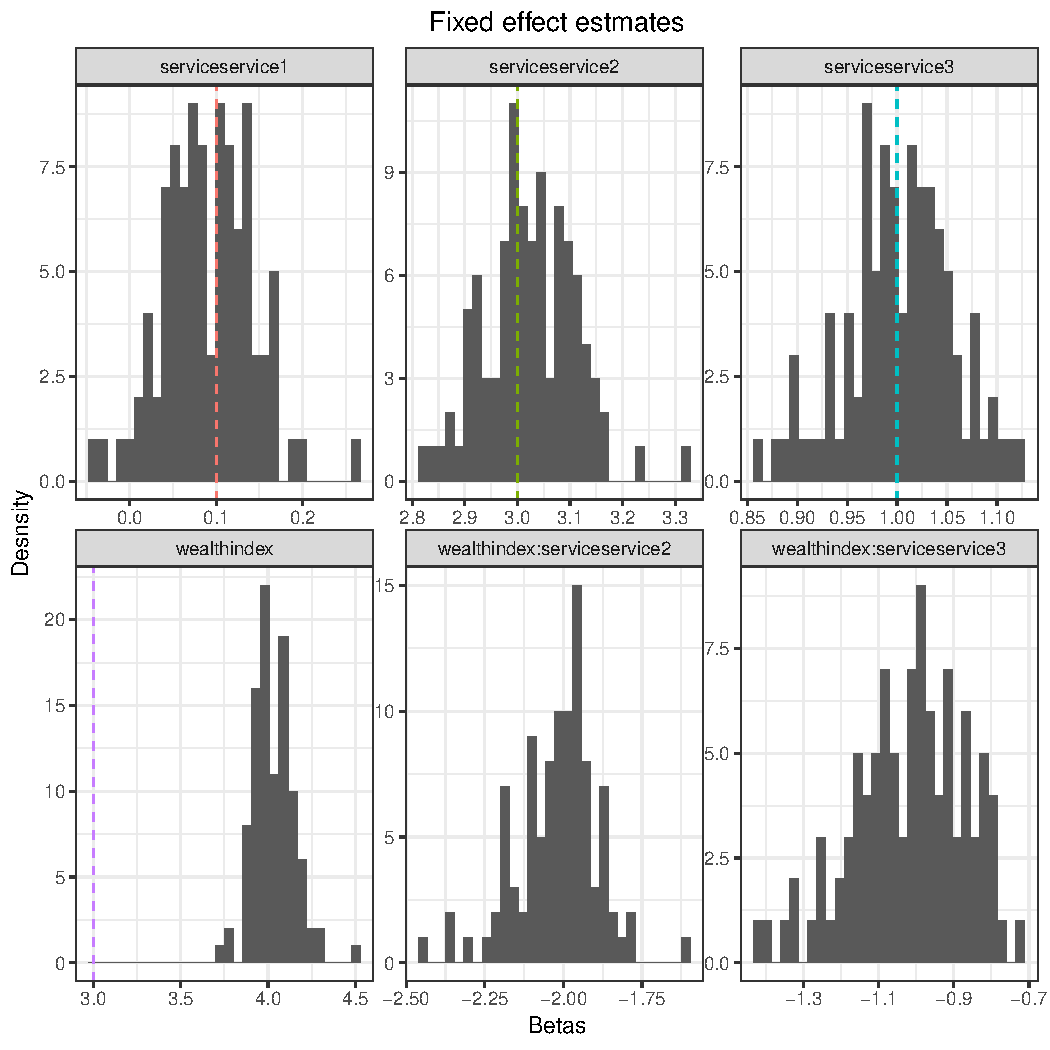
\includegraphics[width=\textwidth]{git_push/glmerSummary.Rout.pdf}
\end{columns}
\item Comments:
\begin{itemize}[<+>]
\item Random slopes for services but not able to capture \textcolor{red}{\textit{true} $\beta$s}
\end{itemize}
\end{itemize}
\end{frame}

\subsection{New Hypothesis}
\begin{frame}{New Hypothesis}
\begin{itemize}[<+->]
\item Discussed the results with \textcolor{blue}{Mac-Theobio} Lab 
\begin{itemize}[<+->]
\item \textcolor{red}{Unidentifiability of latent variability in binary-response models}
\item \textcolor{gray}{Moving to Markov chain Monte Carlo Sampler for Multivariate Generalised Linear Mixed Models}
\end{itemize}
\end{itemize}
\end{frame}

\begin{frame}
\centering
\Huge{\textcolor{blue}{Asanteni Sana}}

\end{frame}
\end{document}
